\documentclass[landscape,twocolumn,letterpaper,9pt,reqno]{article}\usepackage[]{graphicx}\usepackage[]{color}
%% maxwidth is the original width if it is less than linewidth
%% otherwise use linewidth (to make sure the graphics do not exceed the margin)
\makeatletter
\def\maxwidth{ %
  \ifdim\Gin@nat@width>\linewidth
    \linewidth
  \else
    \Gin@nat@width
  \fi
}
\makeatother

\definecolor{fgcolor}{rgb}{0.345, 0.345, 0.345}
\newcommand{\hlnum}[1]{\textcolor[rgb]{0.686,0.059,0.569}{#1}}%
\newcommand{\hlstr}[1]{\textcolor[rgb]{0.192,0.494,0.8}{#1}}%
\newcommand{\hlcom}[1]{\textcolor[rgb]{0.678,0.584,0.686}{\textit{#1}}}%
\newcommand{\hlopt}[1]{\textcolor[rgb]{0,0,0}{#1}}%
\newcommand{\hlstd}[1]{\textcolor[rgb]{0.345,0.345,0.345}{#1}}%
\newcommand{\hlkwa}[1]{\textcolor[rgb]{0.161,0.373,0.58}{\textbf{#1}}}%
\newcommand{\hlkwb}[1]{\textcolor[rgb]{0.69,0.353,0.396}{#1}}%
\newcommand{\hlkwc}[1]{\textcolor[rgb]{0.333,0.667,0.333}{#1}}%
\newcommand{\hlkwd}[1]{\textcolor[rgb]{0.737,0.353,0.396}{\textbf{#1}}}%
\let\hlipl\hlkwb

\usepackage{framed}
\makeatletter
\newenvironment{kframe}{%
 \def\at@end@of@kframe{}%
 \ifinner\ifhmode%
  \def\at@end@of@kframe{\end{minipage}}%
  \begin{minipage}{\columnwidth}%
 \fi\fi%
 \def\FrameCommand##1{\hskip\@totalleftmargin \hskip-\fboxsep
 \colorbox{shadecolor}{##1}\hskip-\fboxsep
     % There is no \\@totalrightmargin, so:
     \hskip-\linewidth \hskip-\@totalleftmargin \hskip\columnwidth}%
 \MakeFramed {\advance\hsize-\width
   \@totalleftmargin\z@ \linewidth\hsize
   \@setminipage}}%
 {\par\unskip\endMakeFramed%
 \at@end@of@kframe}
\makeatother

\definecolor{shadecolor}{rgb}{.97, .97, .97}
\definecolor{messagecolor}{rgb}{0, 0, 0}
\definecolor{warningcolor}{rgb}{1, 0, 1}
\definecolor{errorcolor}{rgb}{1, 0, 0}
\newenvironment{knitrout}{}{} % an empty environment to be redefined in TeX

\usepackage{alltt}

\usepackage{lscape,fancyhdr}

\usepackage{hyperref}

\pagestyle{fancy}

\usepackage{amsmath,epsfig,subfigure,amsthm,amsfonts,epsf,psfrag,rotating,setspace,bm}

\usepackage{verbatim,color} % Allow text colors}

\setlength{\oddsidemargin}{-0.4in}		% default=0in
\setlength\evensidemargin{-0.4in}

\setlength{\textwidth}{9.8in}		% default=9in

\setlength{\columnsep}{0.5in}		% default=10pt

\setlength{\columnseprule}{0pt}		% default=0pt (no line)


\setlength{\textheight}{7.0in}		% default=5.15in

\setlength{\topmargin}{-0.75in}		% default=0.20in

\setlength{\headsep}{0.25in}		% default=0.35in

\setlength{\parskip}{1.2ex}

\setlength{\parindent}{0mm}

\lhead{Course EPIB607: Regression handout 002}
\rhead{jh,sb \ \ \ v. 2018.11.08}
\IfFileExists{upquote.sty}{\usepackage{upquote}}{}
\begin{document}




\section{Mean depth of the ocean}




\begin{knitrout}
\definecolor{shadecolor}{rgb}{0.969, 0.969, 0.969}\color{fgcolor}
\begin{alltt}
\hlkwd{head}\hlstd{(depths)}
\end{alltt}
\begin{verbatim}
##           X        lon       lat  alt water South
## 41995 41995  -87.21236 59.290367  190     1     0
## 11151 11151 -122.33034  5.554558 4167     1     0
## 43640 43640 -148.54790 36.237464 5447     1     0
## 8615   8615  -24.92364 21.625967 5063     1     0
## 8126   8126  177.18458 13.880370 5634     1     0
## 16548 16548   48.88215  3.229250 3691     1     0
\end{verbatim}
\begin{alltt}
\hlkwd{dim}\hlstd{(depths)}
\end{alltt}
\begin{verbatim}
## [1] 400   6
\end{verbatim}
\begin{alltt}
\hlstd{fit} \hlkwb{<-} \hlkwd{lm}\hlstd{(alt} \hlopt{~} \hlnum{1}\hlstd{,} \hlkwc{data} \hlstd{= depths)}
\hlkwd{summary}\hlstd{(fit)}
\end{alltt}
\begin{verbatim}
## 
## Call:
## lm(formula = alt ~ 1, data = depths)
## 
## Residuals:
##     Min      1Q  Median      3Q     Max 
## -3681.5  -584.8   405.5  1197.2  2827.5 
## 
## Coefficients:
##             Estimate Std. Error t value Pr(>|t|)    
## (Intercept)  3683.52      78.71    46.8   <2e-16 ***
## ---
## Signif. codes:  0 '***' 0.001 '**' 0.01 '*' 0.05 '.' 0.1 ' ' 1
## 
## Residual standard error: 1574 on 399 degrees of freedom
\end{verbatim}

\end{knitrout}
	

\clearpage
	
\section{Mean depth of the ocean in northern and southern hemisphere}

\begin{knitrout}
\definecolor{shadecolor}{rgb}{0.969, 0.969, 0.969}\color{fgcolor}

{\centering 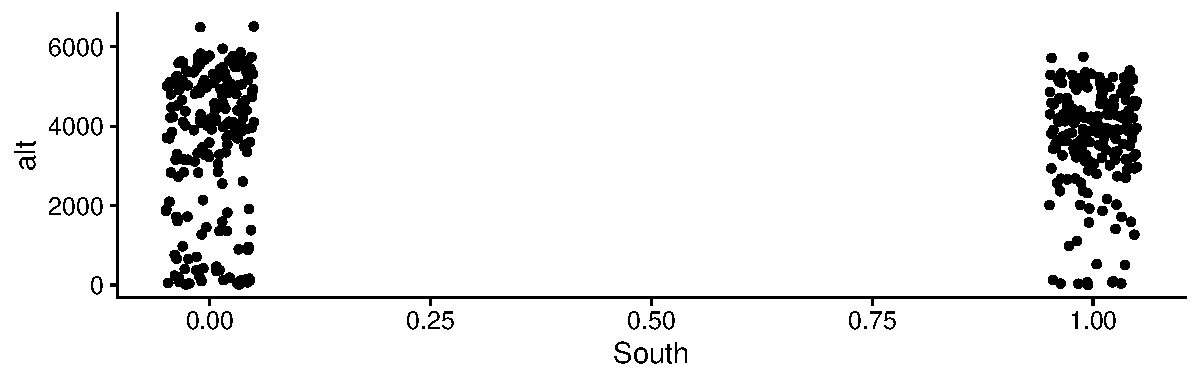
\includegraphics[width=1\linewidth]{figure/unnamed-chunk-3-1} 

}



\end{knitrout}


\begin{knitrout}\footnotesize
\definecolor{shadecolor}{rgb}{0.969, 0.969, 0.969}\color{fgcolor}
\begin{alltt}
\hlstd{fit} \hlkwb{<-} \hlkwd{lm}\hlstd{(alt} \hlopt{~} \hlstd{South,} \hlkwc{data} \hlstd{= depths)}
\hlkwd{summary}\hlstd{(fit)}
\end{alltt}
\begin{verbatim}
## 
## Call:
## lm(formula = alt ~ South, data = depths)
## 
## Residuals:
##     Min      1Q  Median      3Q     Max 
## -3722.0  -608.5   401.5  1200.4  2867.9 
## 
## Coefficients:
##             Estimate Std. Error t value Pr(>|t|)    
## (Intercept)  3643.08     111.42  32.698   <2e-16 ***
## South          80.88     157.56   0.513    0.608    
## ---
## Signif. codes:  0 '***' 0.001 '**' 0.01 '*' 0.05 '.' 0.1 ' ' 1
## 
## Residual standard error: 1576 on 398 degrees of freedom
## Multiple R-squared:  0.0006617,	Adjusted R-squared:  -0.001849 
## F-statistic: 0.2635 on 1 and 398 DF,  p-value: 0.608
\end{verbatim}
\begin{alltt}
\hlkwd{t.test}\hlstd{(alt} \hlopt{~} \hlstd{South,} \hlkwc{data} \hlstd{= depths,} \hlkwc{var.equal} \hlstd{=} \hlnum{TRUE}\hlstd{)}
\end{alltt}
\begin{verbatim}
## 
## 	Two Sample t-test
## 
## data:  alt by South
## t = -0.51334, df = 398, p-value = 0.608
## alternative hypothesis: true difference in means is not equal to 0
## 95 percent confidence interval:
##  -390.6487  228.8787
## sample estimates:
## mean in group 0 mean in group 1 
##        3643.080        3723.965
\end{verbatim}

\end{knitrout}

\clearpage

\section{Ratio depth of the ocean in northern and southern hemisphere}

\begin{knitrout}
\definecolor{shadecolor}{rgb}{0.969, 0.969, 0.969}\color{fgcolor}
\begin{alltt}
\hlcom{# note: we are now using glm}
\hlstd{fit} \hlkwb{<-} \hlkwd{glm}\hlstd{(alt} \hlopt{~} \hlstd{South,} \hlkwc{data} \hlstd{= depths,} \hlkwc{family} \hlstd{=} \hlkwd{gaussian}\hlstd{(}\hlkwc{link}\hlstd{=log))}
\hlkwd{summary}\hlstd{(fit)}
\end{alltt}
\begin{verbatim}
## 
## Call:
## glm(formula = alt ~ South, family = gaussian(link = log), data = depths)
## 
## Deviance Residuals: 
##     Min       1Q   Median       3Q      Max  
## -3722.0   -608.5    401.5   1200.4   2867.9  
## 
## Coefficients:
##             Estimate Std. Error t value Pr(>|t|)    
## (Intercept)  8.20058    0.03058 268.144   <2e-16 ***
## South        0.02196    0.04278   0.513    0.608    
## ---
## Signif. codes:  0 '***' 0.001 '**' 0.01 '*' 0.05 '.' 0.1 ' ' 1
## 
## (Dispersion parameter for gaussian family taken to be 2482673)
## 
##     Null deviance: 988758010  on 399  degrees of freedom
## Residual deviance: 988103771  on 398  degrees of freedom
## AIC: 7029.1
## 
## Number of Fisher Scoring iterations: 5
\end{verbatim}

\end{knitrout}


\clearpage


\section{Student drinking}



\begin{knitrout}\footnotesize
\definecolor{shadecolor}{rgb}{0.969, 0.969, 0.969}\color{fgcolor}
\begin{alltt}
\hlstd{fit} \hlkwb{<-} \hlkwd{lm}\hlstd{(drinks} \hlopt{~} \hlstd{gender,} \hlkwc{data} \hlstd{= drinks)}
\hlkwd{summary}\hlstd{(fit)}
\end{alltt}
\begin{verbatim}
## 
## Call:
## lm(formula = drinks ~ gender, data = drinks)
## 
## Residuals:
##     Min      1Q  Median      3Q     Max 
## -5.5185 -1.7947 -0.2947  1.4815  9.4815 
## 
## Coefficients:
##             Estimate Std. Error t value Pr(>|t|)    
## (Intercept)   4.2947     0.2837  15.138  < 2e-16 ***
## gender        2.2238     0.4182   5.318  3.2e-07 ***
## ---
## Signif. codes:  0 '***' 0.001 '**' 0.01 '*' 0.05 '.' 0.1 ' ' 1
## 
## Residual standard error: 2.765 on 174 degrees of freedom
## Multiple R-squared:  0.1398,	Adjusted R-squared:  0.1348 
## F-statistic: 28.28 on 1 and 174 DF,  p-value: 3.197e-07
\end{verbatim}
\begin{alltt}
\hlstd{fit} \hlkwb{<-} \hlkwd{glm}\hlstd{(drinks} \hlopt{~} \hlstd{gender,} \hlkwc{data} \hlstd{= drinks,} \hlkwc{family} \hlstd{=} \hlkwd{gaussian}\hlstd{(}\hlkwc{link}\hlstd{=log))}
\hlkwd{summary}\hlstd{(fit)}
\end{alltt}
\begin{verbatim}
## 
## Call:
## glm(formula = drinks ~ gender, family = gaussian(link = log), 
##     data = drinks)
## 
## Deviance Residuals: 
##     Min       1Q   Median       3Q      Max  
## -5.5185  -1.7947  -0.2947   1.4815   9.4815  
## 
## Coefficients:
##             Estimate Std. Error t value Pr(>|t|)    
## (Intercept)  1.45739    0.06606  22.062  < 2e-16 ***
## gender       0.41726    0.08115   5.142 7.27e-07 ***
## ---
## Signif. codes:  0 '***' 0.001 '**' 0.01 '*' 0.05 '.' 0.1 ' ' 1
## 
## (Dispersion parameter for gaussian family taken to be 7.646385)
## 
##     Null deviance: 1546.7  on 175  degrees of freedom
## Residual deviance: 1330.5  on 174  degrees of freedom
## AIC: 861.48
## 
## Number of Fisher Scoring iterations: 5
\end{verbatim}

\end{knitrout}









	
	
\end{document}	
